\section{Basics}

\subsection{One-hot encoding}

Throughout this book, we'll often use so-called ``one-hot encoding''.
In short, this is:

\begin{center}
\begin{longtable}{ | l | l | }                                                                    
\hline
Decimal & One-hot \\
\hline
0	& 00000001 \\
1	& 00000010 \\
2	& 00000100 \\
3	& 00001000 \\
4	& 00010000 \\
5	& 00100000 \\
6	& 01000000 \\
7	& 10000000 \\
\hline
\end{longtable}
\end{center}

Or in reversed form:

\begin{center}
\begin{longtable}{ | l | l | }                                                                    
\hline
Decimal & One-hot \\
\hline
0	& 10000000 \\
1	& 01000000 \\
2	& 00100000 \\
3	& 00010000 \\
4	& 00001000 \\
5	& 00000100 \\
6	& 00000010 \\
7	& 00000001 \\
\hline
\end{longtable}
\end{center}

It has several advantages and disadvantages as well.
See also: \url{https://en.wikipedia.org/wiki/One-hot}.

% subsections
\section{\ac{SMT}-solvers}

\subsection{School-level system of equations}

This is school-level system of equations copy-pasted from Wikipedia
\footnote{\url{https://en.wikipedia.org/wiki/System_of_linear_equations}}:

\begin{alignat*}{7}
3x &&\; + \;&& 2y             &&\; - \;&& z  &&\; = \;&& 1 & \\
2x &&\; - \;&& 2y             &&\; + \;&& 4z &&\; = \;&& -2 & \\
-x &&\; + \;&& \tfrac{1}{2} y &&\; - \;&& z  &&\; = \;&& 0 &
\end{alignat*}

Will it be possible to solve it using Z3? Here it is:

\begin{lstlisting}
#!/usr/bin/python
from z3 import *

x = Real('x')
y = Real('y')
z = Real('z')
s = Solver()
s.add(3*x + 2*y - z == 1)
s.add(2*x - 2*y + 4*z == -2)
s.add(-x + 0.5*y - z == 0)
print s.check()
print s.model()
\end{lstlisting}

We see this after run:

\begin{lstlisting}
sat
[z = -2, y = -2, x = 1]
\end{lstlisting}

If we change any equation in some way so it will have no solution, s.check() will return ``unsat''.

I've used ``Real'' \emph{sort} (some kind of data type in \ac{SMT}-solvers)
because the last expression equals to $\frac{1}{2}$, which is, of course, a real number.
For the integer system of equations, ``Int'' \emph{sort} would work fine.

Python (and other high-level \ac{PL}s like C\#) interface is highly popular, because it's practical, but in fact, 
there is a standard language for \ac{SMT}-solvers called SMT-LIB
\footnote{\url{http://smtlib.cs.uiowa.edu/papers/smt-lib-reference-v2.5-r2015-06-28.pdf}}.

Our example rewritten to it looks like this:

\begin{lstlisting}
(declare-const x Real)
(declare-const y Real)
(declare-const z Real)
(assert (=(-(+(* 3 x) (* 2 y)) z) 1))
(assert (=(+(-(* 2 x) (* 2 y)) (* 4 z)) -2))
(assert (=(-(+ (- 0 x) (* 0.5 y)) z) 0))
(check-sat)
(get-model)
\end{lstlisting}

This language is very close to LISP, but is somewhat hard to read for untrained eyes.

Now we run it:

\begin{lstlisting}
% z3 -smt2 example.smt
sat
(model
  (define-fun z () Real
    (- 2.0))
  (define-fun y () Real
    (- 2.0))
  (define-fun x () Real
    1.0)
)
\end{lstlisting}

So when you look back to my Python code, you may feel that these 3 expressions could be executed.
This is not true: Z3Py API offers overloaded operators, so expressions are constructed and passed into the guts of Z3 without any execution
\footnote{\url{https://github.com/Z3Prover/z3/blob/6e852762baf568af2aad1e35019fdf41189e4e12/src/api/python/z3.py}}.
I would call it ``embedded \ac{DSL}''.

Same thing for Z3 C++ API, you may find there ``operator+'' declarations and many more
\footnote{\url{https://github.com/Z3Prover/z3/blob/6e852762baf568af2aad1e35019fdf41189e4e12/src/api/c\%2B\%2B/z3\%2B\%2B.h}}.

Z3 \ac{API}s for Java, ML and .NET are also exist
\footnote{\url{https://github.com/Z3Prover/z3/tree/6e852762baf568af2aad1e35019fdf41189e4e12/src/api}}.\\
\\
Z3Py tutorial: \url{https://github.com/ericpony/z3py-tutorial}.

Z3 tutorial which uses SMT-LIB language: \url{http://rise4fun.com/Z3/tutorial/guide}.

\subsection{Another school-level system of equations}
\label{eq2_SMT}

I've found this somewhere at Facebook:

\begin{figure}[H]
\centering
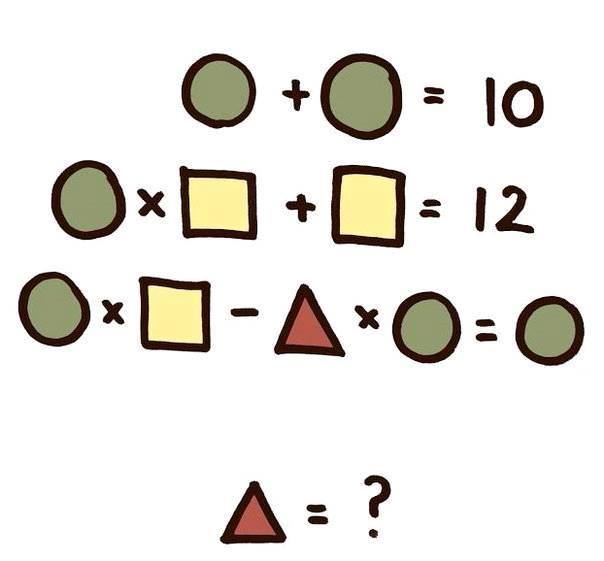
\includegraphics[scale=0.3]{basics/equation.jpg}
\caption{System of equations}
\end{figure}

It's that easy to solve it in Z3:

\begin{lstlisting}
#!/usr/bin/python
from z3 import *

circle, square, triangle = Ints('circle square triangle')
s = Solver()
s.add(circle+circle==10)
s.add(circle*square+square==12)
s.add(circle*square-triangle*circle==circle)
print s.check()
print s.model()
\end{lstlisting}

\begin{lstlisting}
sat
[triangle = 1, square = 2, circle = 5]
\end{lstlisting}

\subsection{Why variables are declared using declare-fun?}

They mean this is nullary function, only returning a constant, nothing else.

\subsection{Connection between \ac{SAT} and \ac{SMT} solvers}

\ac{SMT}-solvers are frontends to \ac{SAT} solvers, i.e.,
they translate inputted SMT expressions into \ac{CNF} and feed SAT-solver with it.
Translation process is sometimes called ``bit blasting''.
Some \ac{SMT}-solvers uses external SAT-solver: STP uses MiniSAT or CryptoMiniSAT as backend.
Some other \ac{SMT}-solvers (like Z3) has their own SAT solver.

\iffalse
\subsection{Theories}

...

QF\_S -- strings. You may need this to simulate strings to catch bugs like SQL injection.
\url{http://cvc4.cs.stanford.edu/wiki/Strings}.
\fi

% subsubsections:
\subsection{List of SMT-solvers}

\begin{itemize}

\item Yices\footnote{\url{http://yices.csl.sri.com/}}, created by Bruno Dutertre et al.

\item Z3\footnote{\url{https://github.com/Z3Prover/z3}},
developed by Leonardo de Moura, Nikolaj Bjorner, Christoph M. Wintersteiger, Lev Nachmanson.

Many examples here uses Python 2.x API for Z3 (AKA Z3Py).
Installation instructions (Ubuntu):

\begin{lstlisting}
sudo apt-get install python3-pip
sudo pip3 install z3-solver
\end{lstlisting}

Or compile the latest on Ubuntu:

\begin{lstlisting}
git clone https://github.com/Z3Prover/z3.git
cd z3
git tag
git checkout z3-4.8.4	# or another version
python scripts/mk_make.py --python
cd build
make
sudo make install
\end{lstlisting}

(Unofficial) bindings:
Haskell\footnote{\url{http://hackage.haskell.org/package/z3}},
Racket\footnote{\url{https://github.com/philnguyen/z3-rkt}},
Ruby\footnote{\url{https://github.com/prove-rs/z3.rs}}.

\item STP\footnote{\url{https://github.com/stp/stp}}, used in KLEE.

\item CVC3/CVC4\footnote{\url{http://cvc4.stanford.edu/}}.

\item Boolector\footnote{\url{http://fmv.jku.at/boolector/}}, developed by Aina Niemetz, Mathias Preiner and Armin Biere.
Known to be fastest bitvector solver.

\item Alt-Ergo\footnote{\url{https://alt-ergo.ocamlpro.com/}}, used in Frama-C.

\item MathSAT\footnote{\url{http://mathsat.fbk.eu/}}. Developed by Alberto Griggio, Alessandro Cimatti and Roberto Sebastiani.

\item veriT\footnote{\url{http://www.verit-solver.org/}}.
Developed by David Déharbe, Pascal Fontaine, Haniel Barbosa.
Lacks bitvectors.

\item toysolver\footnote{\url{https://github.com/msakai/toysolver}} by Masahiro Sakai, written in Haskell.

\item MK85\footnote{\url{https://github.com/DennisYurichev/MK85}}.
Created by Dennis Yurichev, as a toy bit-blaster, supports booleans and bitvectors.

\item dReal: ``An SMT Solver for Nonlinear Theories of the Reals''
\footnote{\url{http://dreal.cs.cmu.edu}, \url{https://github.com/dreal}}.

\end{itemize}

Something else:

\begin{itemize}

\item PySMT: unified Python interface to many SMT solvers: \url{https://pysmt.readthedocs.io/en/latest/}

\item JavaSMT -- Unified Java API for SMT solvers: \url{https://github.com/sosy-lab/java-smt}

\item jSMTLIB -- Another Java API for SMT solvers: \url{http://smtlib.github.io/jSMTLIB/}

\item SBV: SMT Based Verification in Haskell: \url{http://leventerkok.github.io/sbv/}

\end{itemize}


\subsection{Z3 specific}

The output is not guaranteed to be random.
You can randomize it by:

\begin{lstlisting}
import time

...

s=Solver()
set_param("smt.random_seed", int(time.time()))
\end{lstlisting}

Or conversely, you may want to reproduce its result each time the same:

\begin{lstlisting}
set_param("smt.random_seed", 1234)
\end{lstlisting}



\section{\ac{SAT}-solvers}

\renewcommand{\CURPATH}{basics/SAT}

SMT vs. SAT is like high level \ac{PL} vs. assembly language.
The latter can be much more efficient, but it's hard to program in it.

SAT is abbreviation of ``Boolean satisfiability problem''.
The problem is to find such a set of variables, which, if plugged into boolean expression, will result in ``true''.

\subsection{CNF form}

\ac{CNF}\footnote{\url{https://en.wikipedia.org/wiki/Conjunctive_normal_form}} is a \textit{normal form}.

% TODO recheck
% TODO write abt it!
%\textit{normal form} is somewhat similar to polynomials in algebra. 
%What is polynomial?
%It is a standard way to express unsystematic equations like $2x \cdot x$ as $3x$ polynomial, 
%and so you will be able to apply some operations to polynomials like summing, etc.

Any boolean expression can be converted to \textit{normal form} and \ac{CNF} is one of them.
The \ac{CNF} expression is a bunch of clauses (sub-expressions) constisting of terms (variables), ORs and NOTs, 
all of which are then glueled together with AND into a full expression.
There is a way to memorize it: \ac{CNF} is ``AND of ORs'' (or ``product of sums'') and \ac{DNF} is ``OR of ANDs'' (or ``sum of products'').

Example is: $(\neg A \vee B) \wedge (C \vee \neg D)$.

$\vee$ stands for OR (logical disjunction\footnote{\url{https://en.wikipedia.org/wiki/Logical_disjunction}}), 
``+'' sign is also sometimes used for OR.

$\wedge$ stands for AND (logical conjunction\footnote{\url{https://en.wikipedia.org/wiki/Logical_conjunction}}).
It is easy to memorize: $\wedge$ looks like ``A'' letter.
``$\cdot$'' is also sometimes used for AND.

$\neg$ is negation (NOT).

% TODO A/B is the first clause, C/D is second

\subsection{Example: 2-bit adder}
\label{adder}

\ac{SAT}-solver is merely a solver of huge boolean equations in CNF form.
It just gives the answer, if there is a set of input values which can satisfy CNF expression, and what input values must be.

Here is a 2-bit adder for example:

\begin{figure}[ht!]
\centering
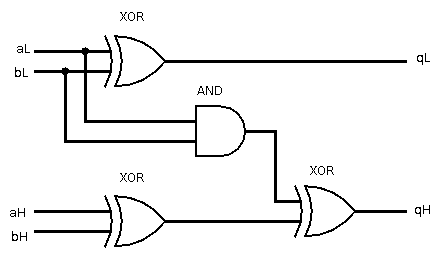
\includegraphics[scale=0.75]{\CURPATH/adder_logisim.png}
\caption{2-bit adder circuit}
\end{figure}

The adder in its simplest form: it has no carry-in and carry-out, and it has 3 XOR gates and one AND gate.
Let's try to figure out, which sets of input values will force adder to set both two output bits?
By doing quick memory calculation, we can see that there are 4 ways to do so: $0+3=3$, $1+2=3$, $2+1=3$, $3+0=3$.
Here is also truth table, with these rows highlighted:

\newcommand{\HLcell}{\cellcolor{blue!25}}

\begin{center}
\begin{doublespace}
\noindent\(\begin{array}{l|llllll}
  & \text{aH} & \text{aL} & \text{bH} & \text{bL} & \text{qH} & \text{qL} \\
\hline
 \text{3+3 = 6 $\equiv $ 2 (mod 4)} & 1 & 1 & 1 & 1 & 1 & 0 \\
 \text{3+2 = 5 $\equiv $ 1 (mod 4)} & 1 & 1 & 1 & 0 & 0 & 1 \\
 \text{3+1 = 4 $\equiv $ 0 (mod 4)} & 1 & 1 & 0 & 1 & 0 & 0 \\
 \text{\HLcell{}3+0 = 3 $\equiv $ 3 (mod 4)} & \HLcell{}1 & \HLcell{}1 & \HLcell{}0 & \HLcell{}0 & \HLcell{}1 & \HLcell{}1 \\
 \text{2+3 = 5 $\equiv $ 1 (mod 4)} & 1 & 0 & 1 & 1 & 0 & 1 \\
 \text{2+2 = 4 $\equiv $ 0 (mod 4)} & 1 & 0 & 1 & 0 & 0 & 0 \\
 \text{\HLcell{}2+1 = 3 $\equiv $ 3 (mod 4)} & \HLcell{}1 & \HLcell{}0 & \HLcell{}0 & \HLcell{}1 & \HLcell{}1 & \HLcell{}1 \\
 \text{2+0 = 2 $\equiv $ 2 (mod 4)} & 1 & 0 & 0 & 0 & 1 & 0 \\
 \text{1+3 = 4 $\equiv $ 0 (mod 4)} & 0 & 1 & 1 & 1 & 0 & 0 \\
 \text{\HLcell{}1+2 = 3 $\equiv $ 3 (mod 4)} & \HLcell{}0 & \HLcell{}1 & \HLcell{}1 & \HLcell{}0 & \HLcell{}1 & \HLcell{}1 \\
 \text{1+1 = 2 $\equiv $ 2 (mod 4)} & 0 & 1 & 0 & 1 & 1 & 0 \\
 \text{1+0 = 1 $\equiv $ 1 (mod 4)} & 0 & 1 & 0 & 0 & 0 & 1 \\
 \text{\HLcell{}0+3 = 3 $\equiv $ 3 (mod 4)} & \HLcell{}0 & \HLcell{}0 & \HLcell{}1 & \HLcell{}1 & \HLcell{}1 & \HLcell{}1 \\
 \text{0+2 = 2 $\equiv $ 2 (mod 4)} & 0 & 0 & 1 & 0 & 1 & 0 \\
 \text{0+1 = 1 $\equiv $ 1 (mod 4)} & 0 & 0 & 0 & 1 & 0 & 1 \\
 \text{0+0 = 0 $\equiv $ 0 (mod 4)} & 0 & 0 & 0 & 0 & 0 & 0 \\
\end{array}\)
\end{doublespace}
\end{center}


Let's find, what \ac{SAT}-solver can say about it?

First, we should represent our 2-bit adder as \ac{CNF} expression.

Using Wolfram Mathematica, we can express 1-bit expression for both adder outputs:\\
\\
\textbf{\texttt{In[]:=AdderQ0[aL$\_$,bL$\_$]=Xor[aL,bL]}} \\
\textbf{\texttt{Out[]:=aL $\veebar$ bL}} \\
\\
\textbf{\texttt{In[]:=AdderQ1[aL$\_$,aH$\_$,bL$\_$,bH$\_$]=Xor[And[aL,bL],Xor[aH,bH]]}} \\
\textbf{\texttt{Out[]:=aH $\veebar$ bH $\veebar$ (aL \&\& bL)}} \\
\\
We need such expression, where both parts will generate 1's.
Let's use Wolfram Mathematica find all instances of such expression (I glueled both parts with And): \\
\\
\textbf{\texttt{In[]:=Boole[SatisfiabilityInstances[And[AdderQ0[aL,bL],AdderQ1[aL,aH,bL,bH]],\{aL,aH,bL,bH\},4]]}} \\
\textbf{\texttt{Out[]:=\{1,1,0,0\},\{1,0,0,1\},\{0,1,1,0\},\{0,0,1,1\}}} \\
\\
Yes, indeed, Mathematica says, there are 4 inputs which will lead to the result we need.
So, Mathematica can also be used as \ac{SAT} solver.

Nevertheless, let's proceed to \ac{CNF} form. Using Mathematica again, let's convert our expression to \ac{CNF} form:\\
\\
\textbf{\texttt{In[]:=cnf=BooleanConvert[And[AdderQ0[aL,bL],AdderQ1[aL,aH,bL,bH]],``CNF'']}} \\
\textbf{\texttt{Out[]:=(!aH $\|$ !bH) \&\& (aH $\|$ bH) \&\& (!aL $\|$ !bL) \&\& (aL $\|$ bL)}} \\
\\
Looks more complex. The reason of such verbosity is that \ac{CNF} form doesn't allow XOR operations.
% FIXME: TeX form of the expression!

\subsubsection{MiniSat}

For starters, we can try MiniSat\footnote{\url{http://minisat.se/MiniSat.html}}.
The standard way to encode \ac{CNF} expression for MiniSat is to enumerate all OR parts at each line.
Also, MiniSat doesn't support variable names, just numbers.
Let's enumerate our variables: 1 will be aH, 2 -- aL, 3 -- bH, 4 -- bL.

Here is what I've got when I converted Mathematica expression to the MiniSat input file:

\lstinputlisting{\CURPATH/adder.cnf}

Two 4's at the first lines are number of variables and number of clauses respectively.
There are 4 lines then, each for each OR clause.
Minus before variable number meaning that the variable is negated.
Absence of minus -- not negated.
Zero at the end is just terminating zero, meaning end of the clause.

In other words, each line is OR-clause with optional negations,
and the task of MiniSat is to find such set of input, which can satisfy all lines in the input file.

That file I named as \textit{adder.cnf} and now let's try MiniSat:

\begin{lstlisting}
% minisat -verb=0 adder.cnf results.txt
SATISFIABLE
\end{lstlisting}

The results are in \textit{results.txt} file:

\begin{lstlisting}
SAT
-1 -2 3 4 0
\end{lstlisting}

This means, if the first two variables (aH and aL) will be \textit{false}, and the last two variables (bH and bL) will be set to \textit{true},
the whole \ac{CNF} expression is satisfiable.
Seems to be true: if bH and bL are the only inputs set to \textit{true}, both resulting bits are also has \textit{true} states.

Now how to get other instances? \ac{SAT}-solvers, like \ac{SMT} solvers, produce only one solution (or \textit{instance}).

MiniSat uses \ac{PRNG} and its initial seed can be set explicitely. I tried different values, but result is still the same.
Nevertheless, CryptoMiniSat in this case was able to show all possible 4 instances, in chaotic order, though.
So this is not very robust way.

Perhaps, the only known way is to negate solution clause and add it to the input expression.
We've got \TT{-1 -2 3 4}, 
now we can negate all values in it (just toggle minuses: \TT{1 2 -3 -4}) and add it to the end of the input file:

\begin{lstlisting}
p cnf 4 5
-1 -3 0
1 3 0
-2 -4 0
2 4 0
1 2 -3 -4
\end{lstlisting}

Now we've got another result:

\begin{lstlisting}
SAT
1 2 -3 -4 0
\end{lstlisting}

This means, aH and aL must be both \textit{true} and bH and bL must be \textit{false}, to satisfy the input expression.
Let's negate this clause and add it again:

\begin{lstlisting}
p cnf 4 6
-1 -3 0
1 3 0
-2 -4 0
2 4 0
1 2 -3 -4
-1 -2 3 4 0
\end{lstlisting}

The result is:

\begin{lstlisting}
SAT
-1 2 3 -4 0
\end{lstlisting}

aH=false, aL=true, bH=true, bL=false. This is also correct, according to our truth table.

Let's add it again:

\begin{lstlisting}
p cnf 4 7
-1 -3 0
1 3 0
-2 -4 0
2 4 0
1 2 -3 -4
-1 -2 3 4 0
1 -2 -3 4 0
\end{lstlisting}

\begin{lstlisting}
SAT
1 -2 -3 4 0
\end{lstlisting}

\textit{aH=true, aL=false, bH=false, bL=true.} This is also correct.

This is fourth result. There are shouldn't be more. What if to add it?

\begin{lstlisting}
p cnf 4 8
-1 -3 0
1 3 0
-2 -4 0
2 4 0
1 2 -3 -4
-1 -2 3 4 0
1 -2 -3 4 0
-1 2 3 -4 0
\end{lstlisting}

Now MiniSat just says ``UNSATISFIABLE'' without any additional information in the resulting file.

Our example is tiny, but MiniSat can work with huge \ac{CNF} expressions.

\subsubsection{CryptoMiniSat}

XOR operation is absent in \ac{CNF} form, but crucial in cryptographical algorithms.
Simplest possible way to represent single XOR operation in \ac{CNF} form is:
$(\neg x \vee \neg y) \wedge (x \vee y)$ -- not that small expression, 
though, many XOR operations in single expression can be optimized better.

One significant difference between MiniSat and CryptoMiniSat is that
the latter supports clauses with XOR operations instead of ORs,
because CryptoMiniSat has aim to analyze crypto algorithms\footnote{\url{http://www.msoos.org/xor-clauses/}}.
XOR clauses are handled by CryptoMiniSat in a special way without translating to OR clauses.

You need just to prepend a clause with ``x'' in \ac{CNF} file and OR clause is then treated as XOR clause by CryptoMiniSat.
As of 2-bit adder, this smallest possible XOR-CNF expression can be used to find all inputs where both output adder bits are set:

$(aH \oplus bH) \wedge (aL \oplus bL)$

This is \TT{.cnf} file for CryptoMiniSat:

\begin{lstlisting}
p cnf 4 2
x1 3 0
x2 4 0
\end{lstlisting}

Now I run CryptoMiniSat with various random values to initialize its \ac{PRNG} \dots

\begin{lstlisting}
% cryptominisat4 --verb 0 --random 0 XOR_adder.cnf
s SATISFIABLE
v 1 2 -3 -4 0
% cryptominisat4 --verb 0 --random 1 XOR_adder.cnf
s SATISFIABLE
v -1 -2 3 4 0
% cryptominisat4 --verb 0 --random 2 XOR_adder.cnf
s SATISFIABLE
v 1 -2 -3 4 0
% cryptominisat4 --verb 0 --random 3 XOR_adder.cnf
s SATISFIABLE
v 1 2 -3 -4 0
% cryptominisat4 --verb 0 --random 4 XOR_adder.cnf
s SATISFIABLE
v -1 2 3 -4 0
% cryptominisat4 --verb 0 --random 5 XOR_adder.cnf
s SATISFIABLE
v -1 2 3 -4 0
% cryptominisat4 --verb 0 --random 6 XOR_adder.cnf
s SATISFIABLE
v -1 -2 3 4 0
% cryptominisat4 --verb 0 --random 7 XOR_adder.cnf
s SATISFIABLE
v 1 -2 -3 4 0
% cryptominisat4 --verb 0 --random 8 XOR_adder.cnf
s SATISFIABLE
v 1 2 -3 -4 0
% cryptominisat4 --verb 0 --random 9 XOR_adder.cnf
s SATISFIABLE
v 1 2 -3 -4 0
\end{lstlisting}

Nevertheless, all 4 possible solutions are:

\begin{lstlisting}
v -1 -2 3 4 0
v -1 2 3 -4 0
v 1 -2 -3 4 0
v 1 2 -3 -4 0
\end{lstlisting}

\dots the same as reported by MiniSat.

\subsection{Picosat}

At least Picosat can enumerate all possible solutions without crutches I just shown:

\begin{lstlisting}
% picosat --all adder.cnf
s SATISFIABLE
v -1 -2 3 4 0
s SATISFIABLE
v -1 2 3 -4 0
s SATISFIABLE
v 1 2 -3 -4 0
s SATISFIABLE
v 1 -2 -3 4 0
s SOLUTIONS 4
\end{lstlisting}

% subsubsections:
\subsubsection{MaxSAT}

MaxSAT problem is a problem where as many clauses should be satisfied, as possible, but maybe not all.

(Usual) clauses which \textit{must} be satisfied, called \textit{hard clauses}.
Clauses which \textit{should} be satisfied, called \textit{soft clauses}.

MaxSAT solver tries to satisfy all \textit{hard clauses} and as much \textit{soft clauses}, as possible.

*.wcnf files are used, the format is almost the same as in DIMACS files, like:

\begin{lstlisting}
p wcnf 207 796 208
208 1 0
208 2 0
208 3 0
208 4 0

...

1 -152 0
1 -153 0
1 -154 0
1 155 0
1 -156 0
1 -157 0
\end{lstlisting}

Each clause is written as in DIMACS file, but the first number if weight.
MaxSAT solver tries to maximize clauses with bigger weights first.

If the weight has \textit{top weight}, the clause is \textit{hard clause} and must always be satisfied.
\textit{Top weight} is set in header.
In our case, it's 208.

Some well-known MaxSAT solvers are Open-WBO\footnote{\url{http://sat.inesc-id.pt/open-wbo}}, etc.


\subsection{List of SAT-solvers}

% TODO authors, URLs

\begin{itemize}

\item MiniSat\footnote{http://minisat.se/}, serving as a base for others

\item PicoSat, PrecoSat, Lingeling. Created by Armin Biere. Plingeling supports multithreading.

\item CryptoMiniSat. Created by Mate Soos for cryptographical problems exploration.
Supports XOR clauses, multithreading.
Has Python API.

\end{itemize}





